\documentclass[12pt]{article}
\usepackage{geometry}
\usepackage{graphicx}
\usepackage{siunitx}
\usepackage{amsmath}
\usepackage{amssymb}
\usepackage{amsfonts}
\usepackage{enumerate}
\usepackage{multirow}
\usepackage{indentfirst}
\usepackage{rotating}
\usepackage{float}
\usepackage{subfigure}
\usepackage{mathtools}
\usepackage{listings}
\usepackage[cache=false]{minted} 
\usepackage{setspace}
\usepackage[breaklinks,colorlinks,linkcolor=black,citecolor=black,urlcolor=black]{hyperref}


\geometry{top=1.1in, bottom=1.1in,left=1in, right=1in}

\setlength{\parindent}{2em}
\linespread{1.2}



\begin{document}

\begin{titlepage}

\newcommand{\HRule}{\rule{\linewidth}{0.2mm}}

\begin{center}


\includegraphics[width=10cm]{logo.png}
\HRule \\[4cm]
\textsc{\large Physics Laboratory}\\
\textsc{\large(Vp141/Vp241)}\\
\vspace{4cm}
\textsc{\Large Linear Fit Tutorial \& Criteria}\\

\vspace{8.3cm}
\HRule

\vspace{-1.45em}

\begin{flushright}
\text{\scriptsize rev 1.1}
\end{flushright}
\end{center}
\text{\scriptsize Edited by: Yao Yuan}
\end{titlepage}

\section{Uncertainty for a sample average}

If we perform n independent measurements of a physical quantity $X$, obtaining a set of results $x_1,x_2,\ldots,x_n$, the average value $\bar{X}$ of $X$ is defined as

\begin{equation}
\bar{X}=\frac{1}{n}\sum_{i=1}^nx_i,
\end{equation}
and the standard deviation for $X$ may be estimated by the quantity

\begin{equation}
s_X=\sqrt{\frac{1}{n-1}\sum_{i=1}^n(x_i-\bar{X})^2}.
\end{equation}

\par The standard deviation for $\bar{X}$ is then

\begin{equation*}
s_{\bar{X}}=\frac{s_X}{\sqrt{n}}=\sqrt{\frac{1}{n}\frac{1}{n-1}\sum_{i=1}^n(x_i-\bar{X})^2}.
\end{equation*}

\par The sample average $\bar{X}$ follows a \textit{Student T Distribution} with \textbf{n-1} degrees of freedom (This will be taught in probabilistic courses). Thus, the Type-A uncertainty with 95\% confidence is calculated as
\begin{equation}
\Delta_A=t_{n-1,0.95}\cdot \frac{s_X}{\sqrt{n}}=\frac{t_{n-1,0.95}}{\sqrt{n}}\cdot s_X.
\end{equation}

With Type-B uncertainty $\Delta_B$ given, you should be able to calculate \textbf{the total uncertainty} $u=\sqrt{\Delta_A^2+\Delta_B^2}$.

\vspace{0.3em}
The values of $t_{n-1,0.95}$ and $t_{n-1,0.95}/\sqrt{n}$ are given in Table 1.

\begin{table}[H]
\centering
\begin{tabular}{c|cccccccccc}
\hline
n &3 &4 &5 &6 &7 &8 &9 &10 &15 &20\\\hline\hline
$t_{n-1,0.95}$ &4.30 &3.18 &2.78 &2.57 &2.45 &2.36 &2.31 &2.26 &2.14 &2.09 \\
$\frac{t_{n-1,0.95}}{\sqrt{n}}$ &2.48 &1.59 &1.204 &1.05 &0.926 &0.834 &0.770 &0.715 &0.553 &0.467\\\hline
\end{tabular}
\caption{The values of $t_{n-1,0.95}$ and $t_{n-1,0.95}/\sqrt{n}$.}
\end{table}


For other values of n that are not included in the table, please refer to the table at the end of this document for (two-sided) t-values, using two parameters \textbf{n-1} and \textbf{0.95}.
\\

$^*$\textbf{Note} that this is a brief summary for calculation of confidence interval for \textit{sample average}. For more details, please refer to \textbf{``handbook-uncertainty analysis.pdf'' page 8-9}. Also, this is aim to make it clear that the confidence interval for sample average is different from the confidence interval for \textit{linear regression}, which will be explained in the next section.

\section{Uncertainty for a linear fit}

Typically, a linear fit is performed using software such as \textit{Origin, Matlab or Microsoft Excel}. The uncertainty(,which leads to a confidence interval) could be directly obtained from the output. Mostly, we would like to know the uncertainty of the slope.

First, we should know that the slope in a simple linear regression follows a \textit{Student T Distribution} with \textbf{n-2} degrees of freedom

The values of $t_{n-2,0.95}$ are given in Table 2.

\begin{table}[H]
\centering
\begin{tabular}{c|cccccccccc}
\hline
n &3 &4 &5 &6 &7 &8 &9 &10 &15 &20 \\\hline\hline
$t_{n-2,0.95}$ & 12.71 &4.30 &3.18 &2.78 &2.57 &2.45 &2.36 &2.31 &2.16 &2.10 \\\hline
\end{tabular}
\caption{The values of $t_{n-2,0.95}$.}
\end{table}


For other values of n that are not included in the table, please refer to the table at the end of this document for (two-sided) t-values, using two parameters \textbf{n-2} and \textbf{0.95}.
\\

Let us consider a set of sample data for a linear fit, where $n=12$.


\begin{table}[h]
\centering
\begin{tabular}{cc|cc}
\hline
$t_i\,[s]$ &$s_i\,[m]$ &$t_i\,[s]$ &$s_i\,[m]$
\\\hline\hline
1.0  &110  &7.0   &139
\\
2.0  &115   &8.0   &144   
\\
3.0  &120   &9.0   &149   
\\
4.0  &125   &10.0  &154   
\\
5.0  &129   &11.0  &159   
\\
6.0  &134   &12.0  &164  \\

\hline
\end{tabular}
\caption{Sample data for s-t linear fit.}
\end{table}

\begin{table}[h]
\centering
\begin{tabular}{l|l}

\hline
Time $t_i$ [$s$]& $\pm$ 0.1 [$s$] \\\hline
Distance $s_i$ [$m$]& $\pm$ 1 [$m$]\\
\hline
\end{tabular}
\caption{Uncertainty of the measurement (used for error bar drawing).}
\end{table}

Then $n-2=12-2=10$ and the $t_{10,0.95}=2.228$ is read from the table in appendix.

\newpage
\subsection{OriginLab}

First, import the data, make sure you have included all X, Y, X error and Y error, otherwise you won't have error bars in the plot.

\begin{figure}[H]
\centering
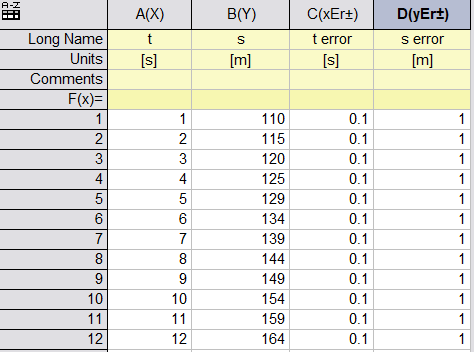
\includegraphics[width=8cm]{o1.png}
\caption{Import data.}
\end{figure}

Then, select all the data and select \textsf{Linear Fit} in menu.

\begin{figure}[H]
\centering
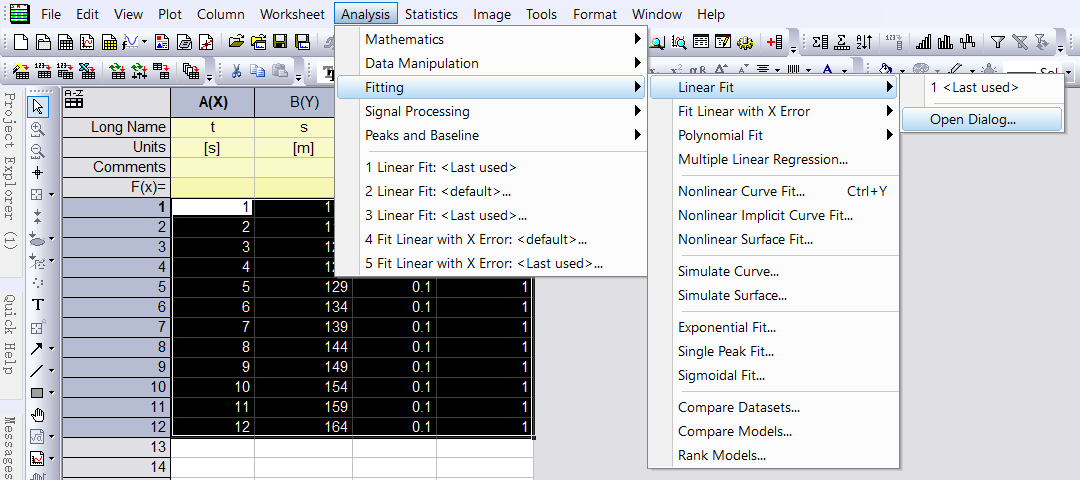
\includegraphics[width=16cm]{o2.png}
\caption{Select linear fit.}
\end{figure}

\newpage

In this menu, tick the quantities as is shown in the figure below, including the necessary \textbf{Standard Error (Standard Deviation), Lower Confidence Limit (LCL), Upper Confidence Limit(UCL), Pearson's r (Correlation Coefficient) and R-Square. 
}Some of them will be included in your report if specified.
\begin{figure}[H]
\centering
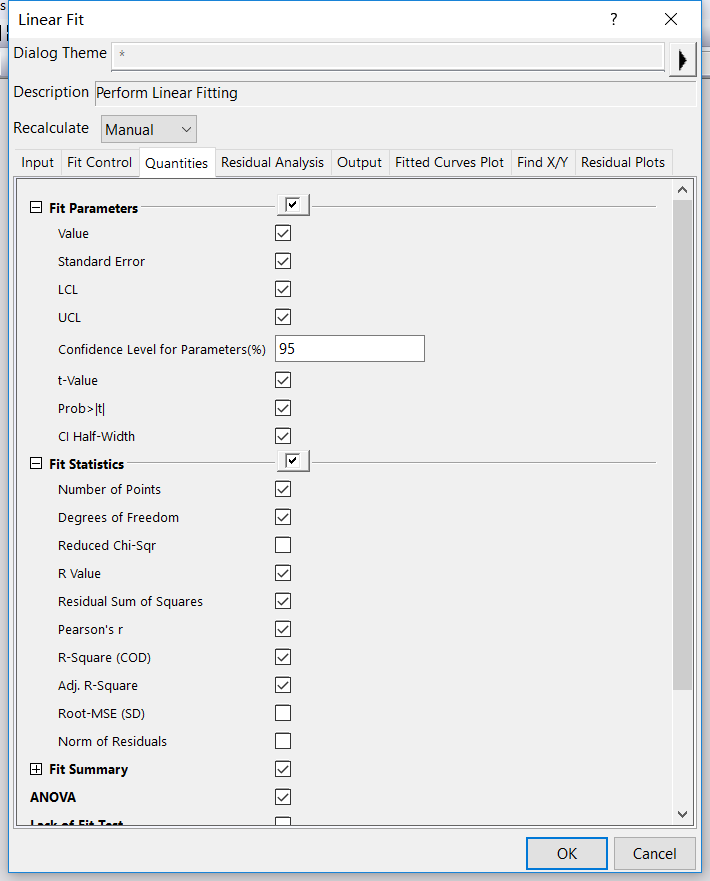
\includegraphics[width=14cm]{o3.png}
\caption{Select quantity display.}
\end{figure}

\newpage

\begin{figure}[H]
\centering
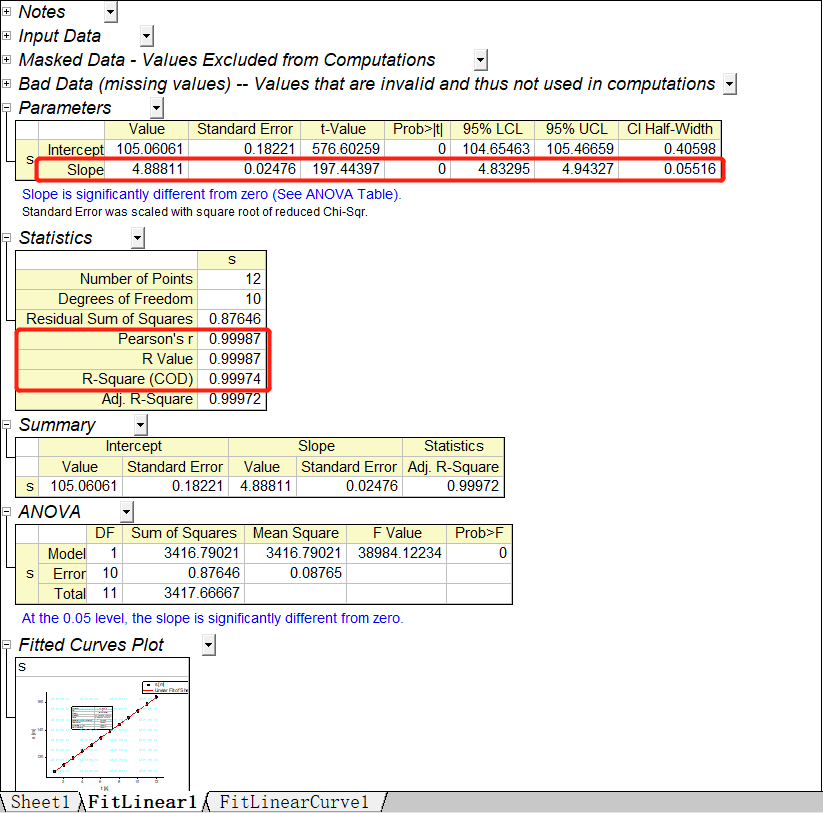
\includegraphics[width=15cm]{o4.png}
\caption{Summary chart.}
\end{figure}

Click OK and you will get this table including all the information you need. Here, the \textbf{CI}(Confidence Interval) \textbf{Half-Width} is the value of \textbf{uncertainty}.

You should notice that the uncertainty (0.05516) is the standard error (0.02476) times $t_{10,0.95}=2.228$. Round the uncertainty to 0.06, and you obtain the uncertainty for the slope.

\newpage
\subsection{Matlab}

To do linear fit in \textsf{Matlab}, you need to acquire \textsf{Curve Fitting} in \textsf{APP}. If you don't have this toolbox, click ``Acquire more App'' on the left and download it(probably need VPN).

\begin{figure}[H]
\centering
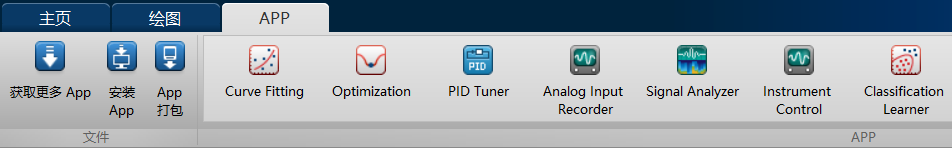
\includegraphics[width=15cm]{m0.png}
\caption{Curve fitting toolbox.}
\end{figure}

Import your data into two matrix variables.

\begin{figure}[H]
\centering
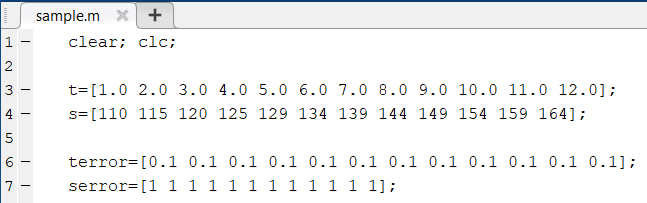
\includegraphics[width=12cm]{m1.png}
\caption{Import data.}
\end{figure}

\newpage
Select \textsf{x data} and \textsf{y data} and parameters will be shown in the ``Results'' window.

\begin{figure}[H]
\centering
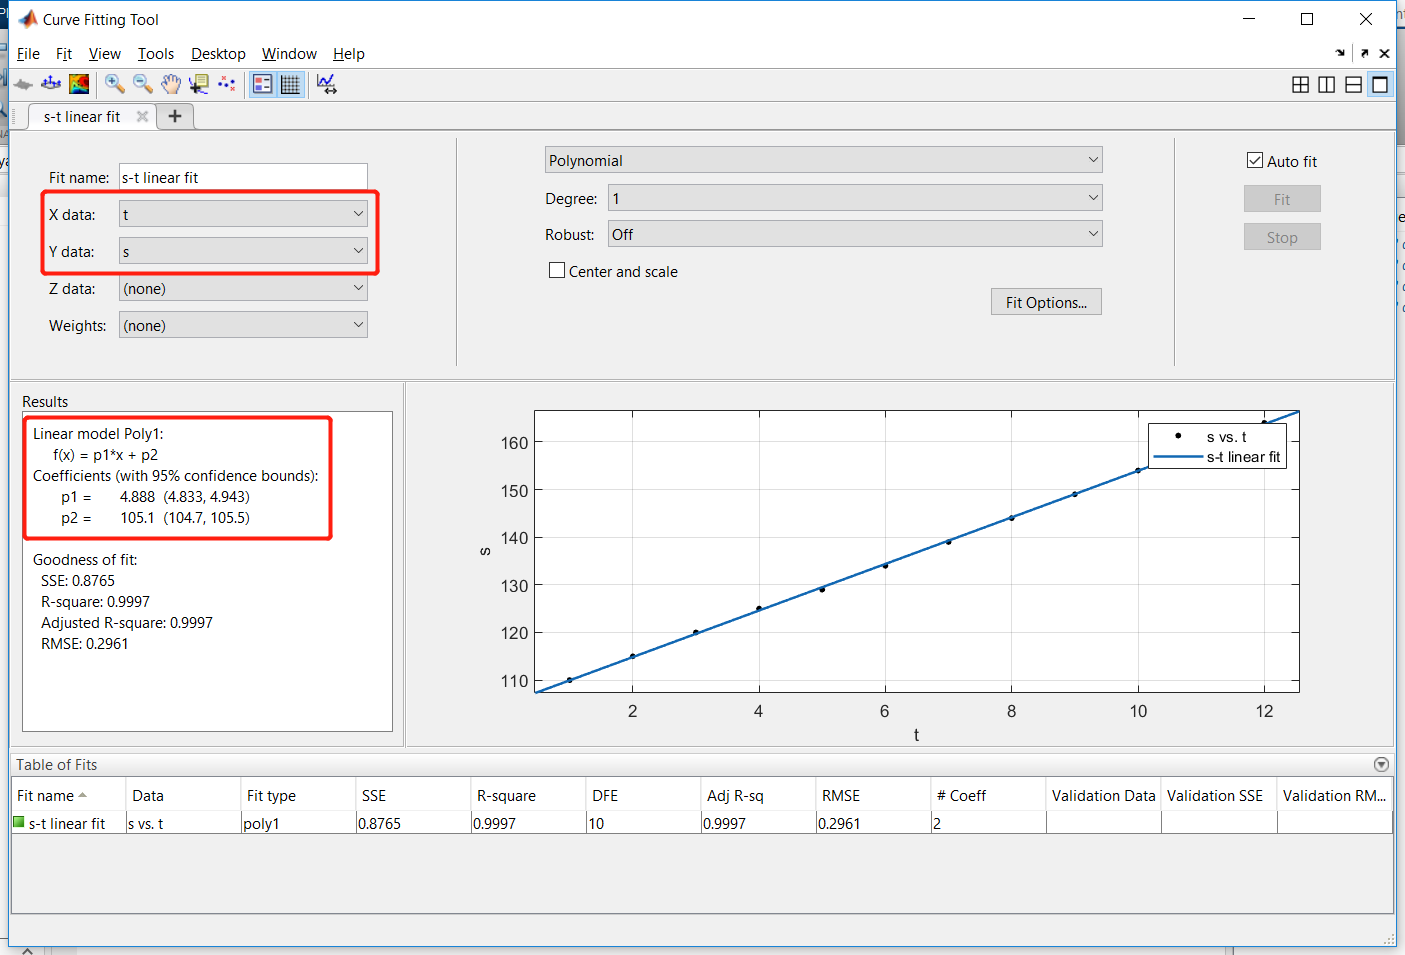
\includegraphics[width=15cm]{m2.png}
\caption{Display settings.}
\end{figure}

As we can see, ``p1'' is the slope we need and its 95\% confidence is given. Divide the length of confidence interval by 2, we obtain the uncertainty (4.943-4.833)/2=0.055$\approx$0.06.

However, the standard error is not given and we can obtain it by dividing the uncertainty by $t_{10,0.95}$.

Furthermore, error bars can be drawn on the plot if you use properly \textsf{hold on} and function \textsf{errorbar}. The remaining tasks are left to you.


\newpage
\subsection{Excel}

First, import all the data you got. 

\begin{figure}[H]
\centering
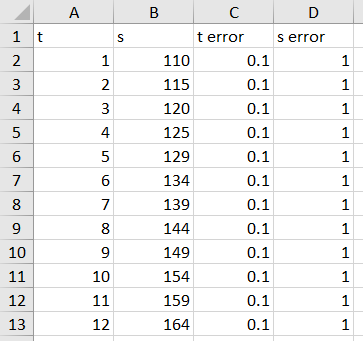
\includegraphics[width=8.4cm]{e0.png}
\caption{Import data.}
\end{figure}

The following steps show how to find the \textsf{Data Analysis} toolbox necessary for a linear regression in \textsf{Excel}.

\begin{figure}[H]
\centering
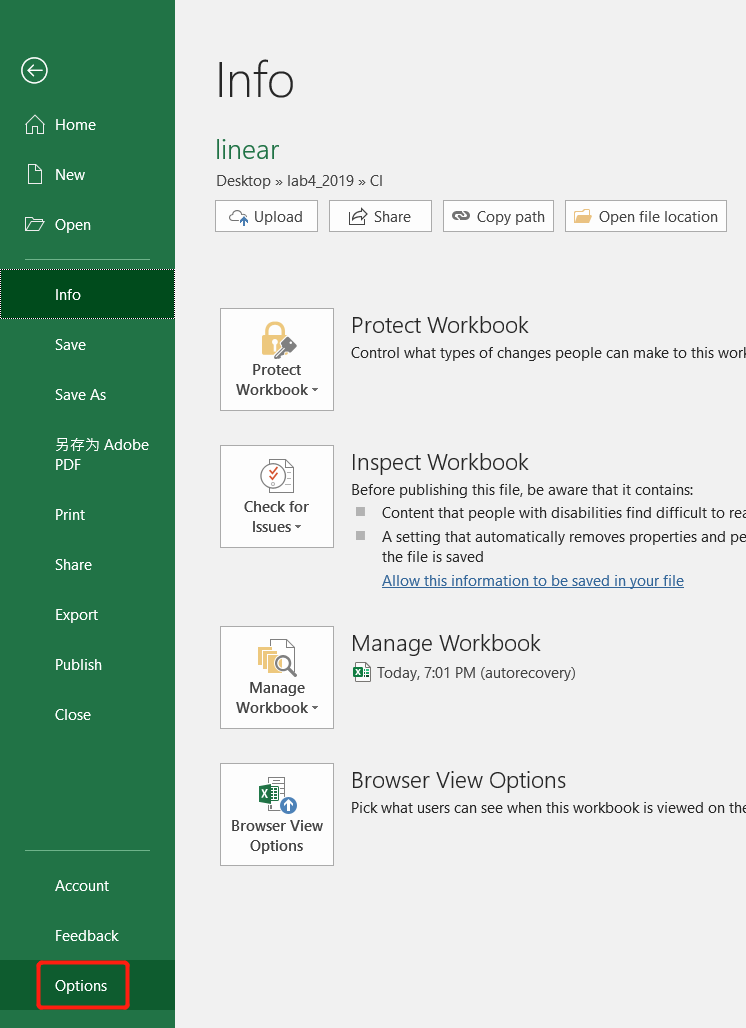
\includegraphics[width=8.4cm]{e4.png}
\caption{File -$>$ Options.}
\end{figure}

\begin{figure}[H]
\centering
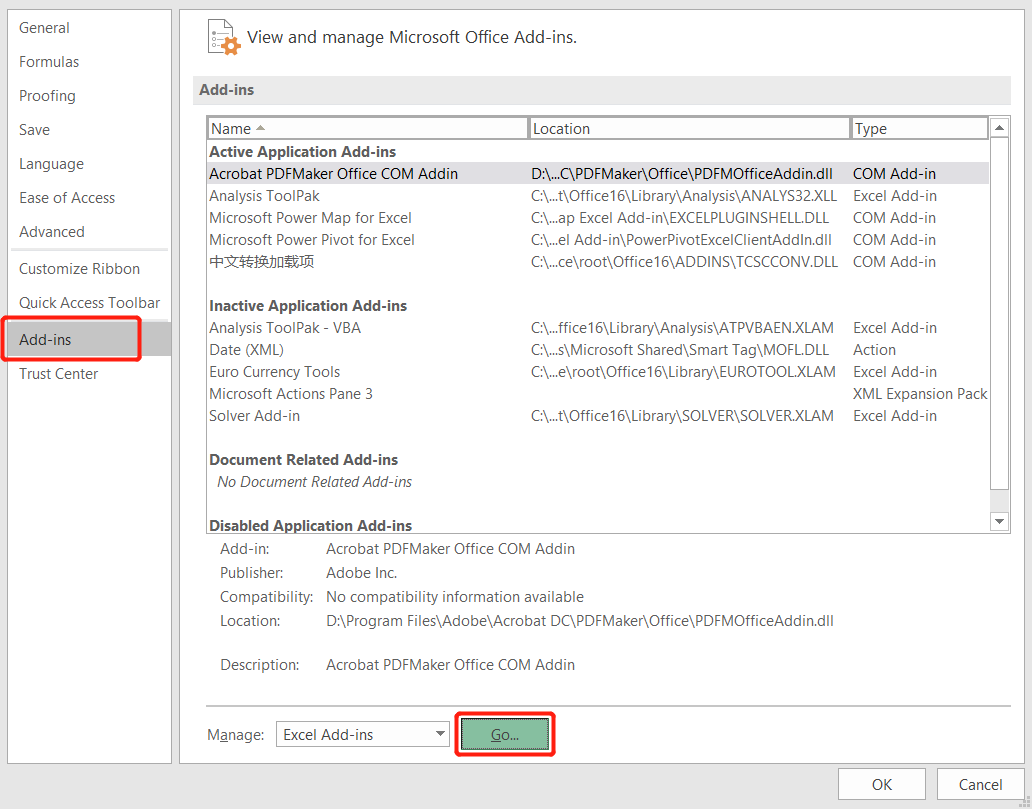
\includegraphics[width=8cm]{e5.png}
\caption{Add-ins -$>$ Go.}
\end{figure}

\begin{figure}[H]
\centering
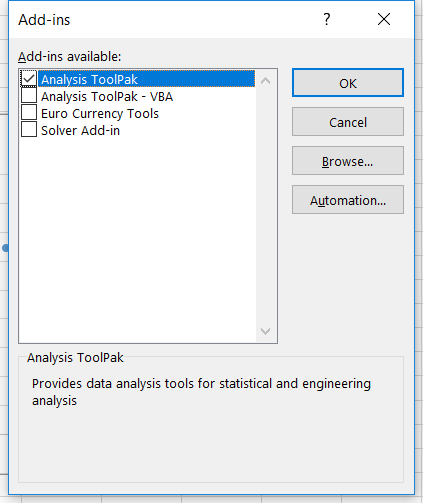
\includegraphics[width=8cm]{e6.png}
\caption{Analysis toolpak.}
\end{figure}

After this, the toolbox will appear in tab \textsf{Data}.

\begin{figure}[H]
\centering
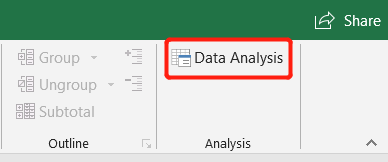
\includegraphics[width=8cm]{e12.png}
\caption{Data analysis.}
\end{figure}

\begin{figure}[H]
\centering
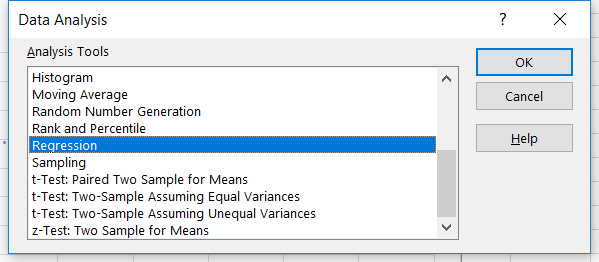
\includegraphics[width=8cm]{e7.png}
\caption{Regression.}
\end{figure}

\begin{figure}[H]
\centering
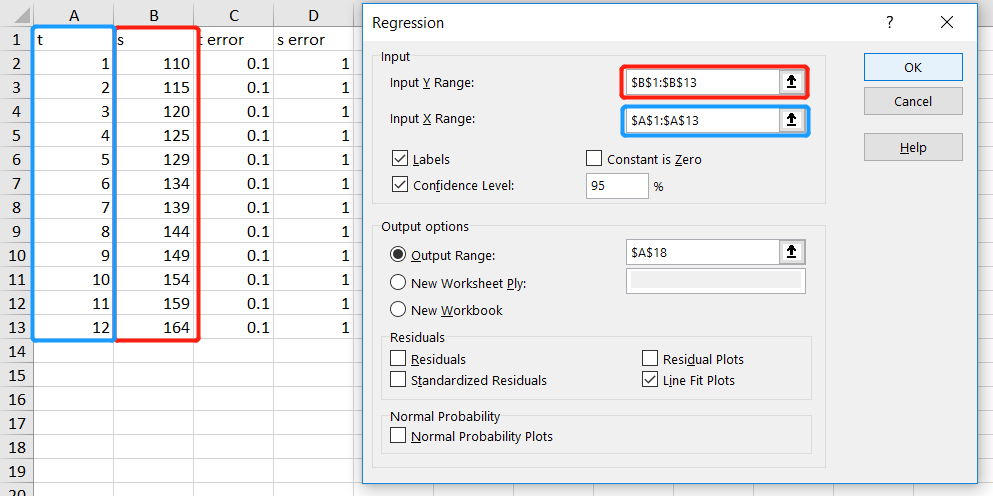
\includegraphics[width=16cm]{e8.png}
\caption{Regression settings.}
\end{figure}

Use this toolbox and you should get all the quantities you need. 

\begin{figure}[H]
\centering
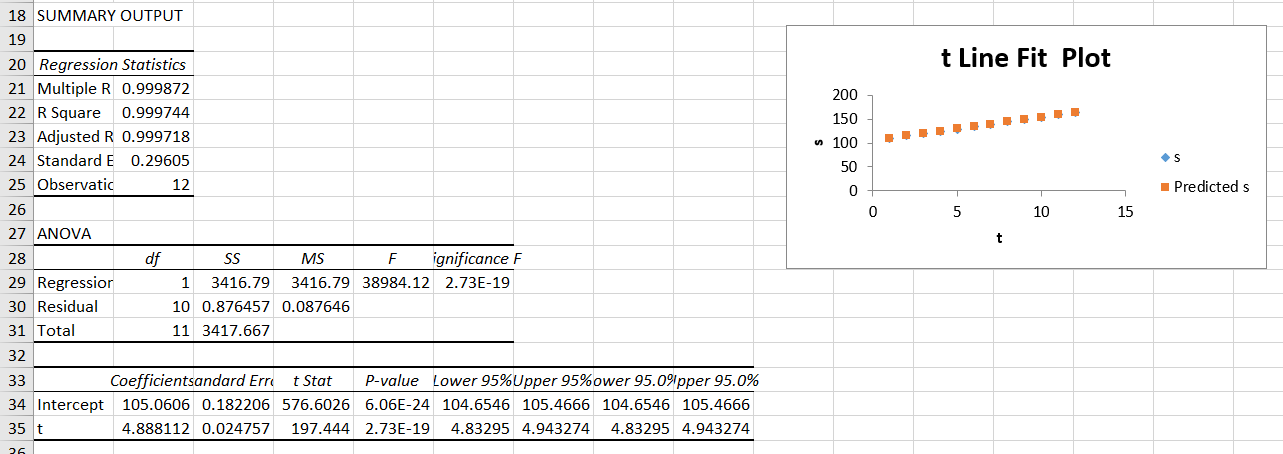
\includegraphics[width=16cm]{e9.png}
\caption{Summary output.}
\end{figure}

Then, the uncertainty can be obtained by
\begin{equation*}
u=t_{10,0.95}\cdot \text{``Standard Error''}=2.228\times0.024757=0.5516\approx0.06.
\end{equation*}

\begin{figure}[H]
\centering
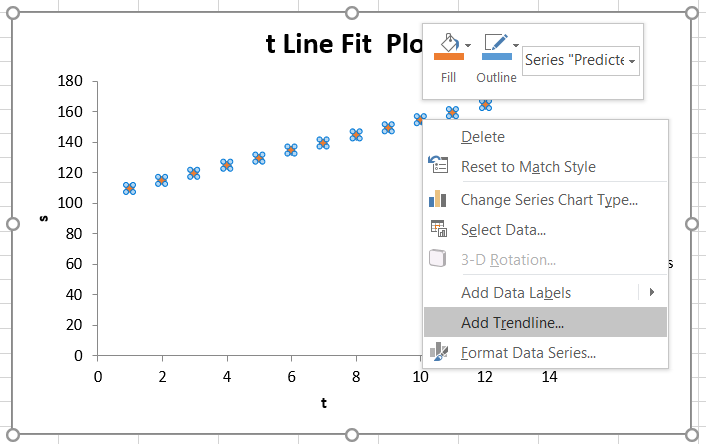
\includegraphics[width=14cm]{e2.png}
\caption{Plot.}
\end{figure}

Also, you will get a fit line by choosing \textsf{Add Trendline}. The remaining tasks are left to you, including adding error bars, a summary chart and legends in the plot.

\vspace{4em}


\subsection{Other Software}

\par For other software, please tell apart standard error and confidence interval(uncertainty). If only one of them is given, calculate another using the same method given above.
\newpage

\section{Sample Plot}

The linear fit plot included in your report should look like this. Of course \textbf{it should have different looks depending on which software you use}, but please make sure that the elements are included.

\begin{figure}[H]
\centering
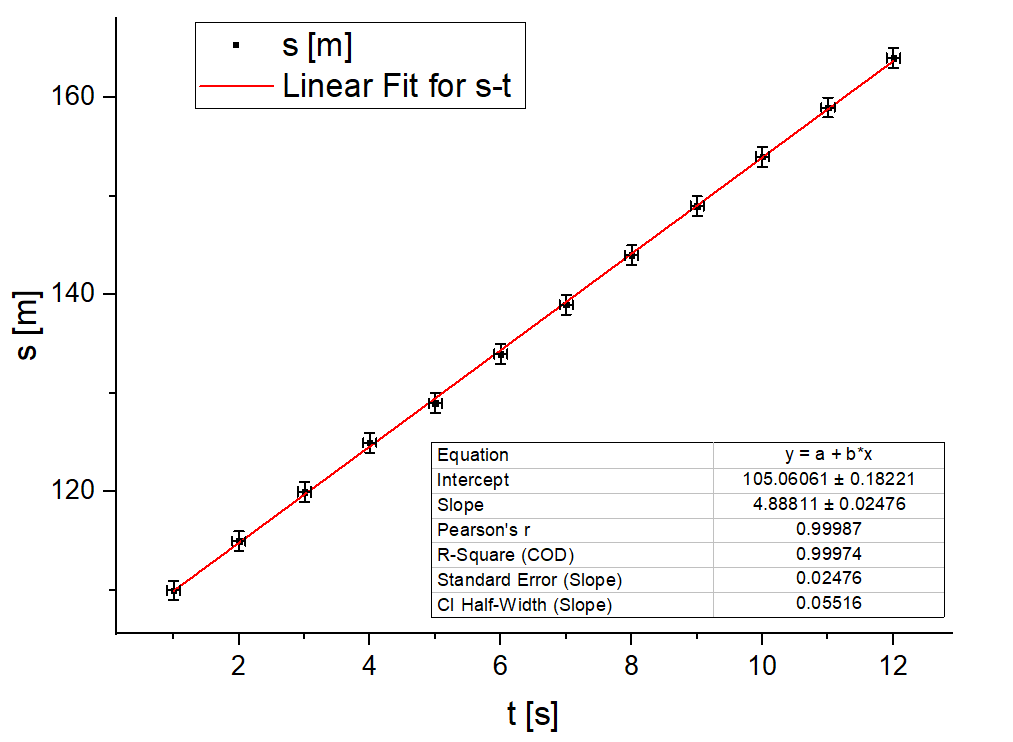
\includegraphics[width=12cm]{sample.png}
\caption{Sample Plot.}
\end{figure}

\vspace{-1em}
\paragraph{Checklist:}\
\par\quad 1. The \textbf{fit line}.
\par\quad 2. \textbf{Data points}.
\par\quad 3. \textbf{Error bars} in both directions. 

(The ones that look like ``H''. Sometimes one set of data is constant and we only have error bars in the other direction. \textit{Must be visible when printed out!!!})
\par\quad 4. Proper \textbf{legends and labels.}
\par\quad 5. \textbf{Summary chart}
\par\qquad\quad Equation
\par\qquad\quad Intercept and Slope
\par\qquad\quad Standard Error {\footnotesize (of the quantity we need)}
\par\qquad\quad Confidence Interval Half-Width {\footnotesize (of the quantity we need)}
\par\qquad\quad Pearson's r
\par\qquad\quad R-Square
\newpage
\section{Appendix}



\begin{figure}[H]
\centering
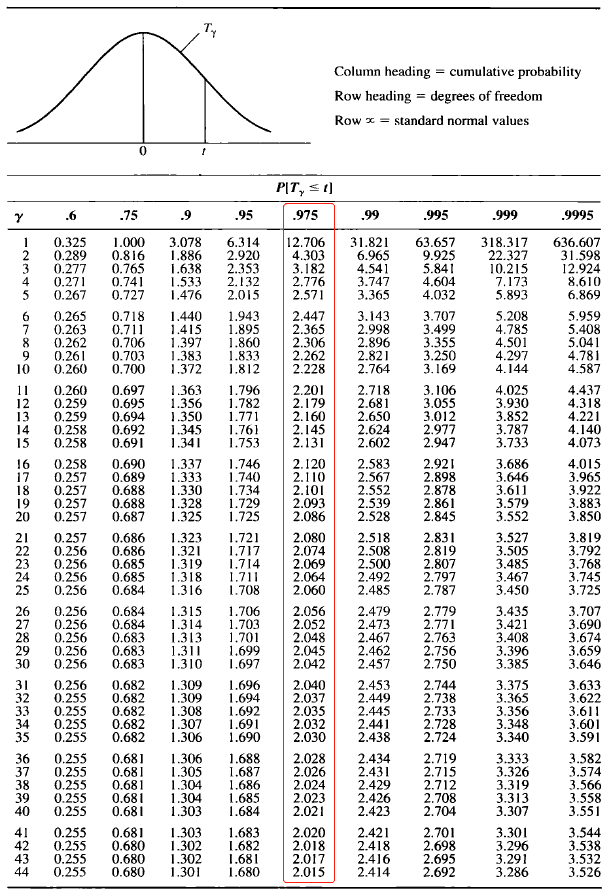
\includegraphics[width=13cm]{ttable.png}
\caption{Table for t-values. Two-sided $t_{0.95}$ values are expressed as one-sided $t_{0.975}$ values, which we choose to use. }

\end{figure}


The table is taken from \textit{Introduction to Probability and Statistics Principles and Application for Engineering and Computer Sciences}.

\end{document}